% PREAMBLE ====================================================================
\PassOptionsToPackage{table}{xcolor}
\documentclass[conference]{IEEEtran}

\usepackage[utf8]{inputenc}
\usepackage[T5]{fontenc}
\usepackage{cite}
\usepackage{textcomp}
\usepackage{graphicx}
\usepackage{amsmath,amssymb,amsfonts}
\usepackage{algorithmic}
\usepackage{xcolor}
\usepackage{float}
\usepackage{booktabs}
\usepackage{tikz}
% \usepackage[english]{babel}
\usepackage{multirow}
\usepackage{tabularx}
\usepackage{makecell}
\usepackage{pgfplots}
\usepackage{balance}
\usepackage{bm}
\usepackage{url}
\usepackage{hyperref}
\usepackage{enumitem}
\usepackage[nameinlink,noabbrev]{cleveref}

\pgfplotsset{compat=1.18}
\usetikzlibrary{shapes.geometric,arrows.meta,positioning,fit,
                backgrounds,calc,decorations.pathreplacing,patterns,shadows}

% ── Colours ──────────────────────────────────────────────────────────────────
\definecolor{C_slate}{RGB}{71,85,105}     \definecolor{C_blue}{RGB}{59,130,246}
\definecolor{C_indigo}{RGB}{99,102,241}   \definecolor{C_amber}{RGB}{245,158,11}
\definecolor{C_rose}{RGB}{244,63,94}      \definecolor{C_sky}{RGB}{14,165,233}
\definecolor{C_bglight}{RGB}{248,250,252} \definecolor{C_bgmid}{RGB}{241,245,249}
\definecolor{C_emerald}{RGB}{16,185,129}  \definecolor{negcol}{RGB}{16,185,129}
\definecolor{C_violet}{RGB}{139,92,246}   \definecolor{C_fuchsia}{RGB}{200,50,220}
\definecolor{headcol}{RGB}{30,41,59}

\newcommand{\NV}{\text{NV}}
\newcommand{\TD}{\text{TD}}
\newcommand{\BKS}{\text{BKS}}

% =============================================================================
\begin{document}

% FIX 1: Restored real title (was Vietnamese joke placeholder)
\title{Optimizing Operator Selection in ALNS using Double DQN\\
       for the VRPTW Problem}

\author{%
  \IEEEauthorblockN{%
    Huynh Nhat Huy\IEEEauthorrefmark{1},
    Nguyen Nhat Huy\IEEEauthorrefmark{1},
    Nguyen Thi Bao Tran\IEEEauthorrefmark{1}}
  \IEEEauthorblockA{%
    \textit{Faculty of Information Technology,
    Ton Duc Thang University, Ho Chi Minh City, Vietnam}}
  \\\small{Advisor: Dr.~Ho Thi Linh}}
\maketitle

% =============================================================================
%  ABSTRACT
% =============================================================================
\begin{abstract}
Static roulette-wheel operator selection limits Adaptive Large Neighborhood Search
(ALNS)~\cite{Ropke2006} to myopic, segment-bounded weight updates, causing
premature convergence on tightly constrained Vehicle Routing Problem with
Time Windows (VRPTW) instances~\cite{Dantzig1959}.

We propose \textbf{Hybrid DDQN-ALNS}: a hierarchical dual-agent framework
coupling a macro \emph{Plateau Controller} with a micro
\emph{Operator Controller} as a Hierarchical Markov Decision Process.  Simulated
Annealing acceptance is replaced by a \emph{Learned Acceptance Criterion} (LAC),
while a \emph{Welford Reward Normalizer}~\cite{welford1962} enables stable
training across a three-stage Domain Randomization Curriculum~\cite{tobin2017domain}.

On 56 Solomon 100-customer and 6 Gehring--Homberger 200-customer instances,
Hybrid DDQN-ALNS reduces mean vehicle inflation to $+0.139$ above BKS on Solomon---a
$\mathbf{13.3\%}$ improvement over ALNS-Base ($+0.161$) and $\mathbf{92.7\%}$ over
OR-Tools ($+1.911$).  NV-filtered travel distance improves by
$\mathbf{5.8\%}$ on wide-horizon families under fair intersection, driven by state-conditioned sequence
polishing.  All results use zero-shot transfer from synthetic training data.
\end{abstract}

\begin{IEEEkeywords}
VRPTW, Adaptive Large Neighborhood Search, Deep Reinforcement Learning,
Hierarchical MDP, Operator Selection.
\end{IEEEkeywords}


% =============================================================================
%  I.  INTRODUCTION
% =============================================================================
\section{Introduction}
\label{sec:intro}

The Vehicle Routing Problem with Time Windows (VRPTW) generalizes the classical Vehicle Routing Problem (VRP) by requiring each customes to be served within a predefined arrival window, transforming an already NP-Hard combitional problem into one where spatial and spatial feasibility must be sastified simultaneously \cite{Dantzig1959, Solomon1987}.
The objective is lexicographic: solvers must minimize the number of vehicles deployed, and only secondary minimizes the travel distance. This ordering reflects the real-world fleet economics, where the fixed cost of an additional vehicle typically dominates the marginal routing distance costs by order of magnitude.

Adaptive Large Neighborhood Search has emerged as one of the most effective metaheuristics framework for VRPTW, owing to it destroy-and repair paradigm and the ability to escape local optima through diversified neighborhood exploration \cite{shaw1998using, Ropke2006, pisinger2007general}. However, the standard ALNS formulation relies on a roulette wheel mechanism for operator selection, where each destroy and repair operator is chosen probabilistically according to weights updated from recent performance. This mechanism suffers from three structural limitations that becomes particulary acute on tightly time-windowed instances.

First, the roulete wheel selection is myopic: adpating weights based on a short historical window without modelling the current search state, so it cannot distinguish between an operator that is generally effective and one that is particually effective specifically given the route topology.
Second, ALNS is prone to  premature plateau convergance, particually on instances where reducing the vehicle count requires tempoarily degrading solution quality - a solution that purely greedy or weighted random-selection rarely discovers unaided.
Third, the simulated annealing acceptance criterion conventionally paired with ALNS uses a globally defined temperature

End-to-end neural approaches---Pointer Networks~\cite{vinyals2015pointer},
attention models~\cite{kool2019attention}, and RL
policies~\cite{nazari2018reinforcement}---demonstrate strong performance on
unconstrained VRP variants but generally optimize weighted objectives rather
than explicitly enforcing lexicographic fleet minimization, and they offer
limited interpretability of the learned search policy.
Our framework closes both gaps by embedding Dueling
DDQN~\cite{wang2016dueling} inside ALNS, preserving hard feasibility while
learning a state-conditioned operator selection policy.

\textbf{Contributions:}
\begin{itemize}[leftmargin=1.2em,topsep=2pt]
  \item \textbf{Hierarchical MDP:} Plateau Controller (macro) and Operator
        Controller (micro) acting as coordinated DDQN agents.ư
  \item \textbf{Learned Acceptance Criterion:} hindsight-labelled binary
        classifier replaces static SA temperature schedules.
  \item \textbf{Welford Normalization~\cite{welford1962}:} online reward
        Z-scoring (${\pm}8\sigma$) enabling stable multi-scale curriculum training.
  \item \textbf{Empirical validation:} 56 Solomon + 6 Gehring--Homberger instances
        with NV-filtered distance reporting, family-level decomposition, and
        Wilcoxon significance tests.
\end{itemize}


A separate line of research has pursued end-to-end neural approaches to vehicle routing, including Pointer Networks [vinyals2015pointer], attention-based construction policies [kool2019attention], and reinforcement learning agents trained to directly output routing decisions [nazari2018reinforcement]. These methods demonstrate that learned policies can capture rich structural regularities in routing problems and generalize across instance distributions. However, they are predominantly designed around scalar or weighted-sum objectives rather than the strict lexicographic fleet-then-distance ordering that VRPTW demands, and they typically function as opaque end-to-end solvers, offering limited visibility into *why* a particular routing decision was made—an important consideration for operational deployment where dispatchers must be able to audit and override automated decisions.

This paper addresses both gaps by embedding a learned, hierarchical decision-making policy directly inside the ALNS search loop rather than replacing the metaheuristic outright. We preserve the hard feasibility guarantees and interpretable operator structure of ALNS, while replacing its static selection and acceptance mechanisms with components trained via reinforcement learning. The result is a search procedure that retains the auditability of classical operations research—every move remains a named destroy or repair operator applied to an explicit route structure—while gaining the adaptivity of a learned policy that conditions its decisions on the live search state.

**Contributions.** This work makes the following contributions:

- We introduce a **Hierarchical Markov Decision Process** formulation for ALNS operator selection, in which a macro-level Plateau Controller selects among coarse search regimes while a micro-level Operator Controller selects destroy-repair operator pairs conditioned on the active regime, both implemented as coordinated Dueling Double DQN agents.

- We replace the conventional simulated annealing acceptance criterion with a **Learned Acceptance Criterion**, a lightweight classifier trained online via hindsight labeling to predict whether accepting a candidate transition—including degrading ones—leads to downstream improvement within a bounded search horizon.

- We identify and resolve a **feasibility entrapment** mechanism that traps strict-feasibility ALNS at vehicle counts above the best-known solution, by introducing penalty-based search over temporarily infeasible intermediate states, combined with structural local search operators (inter-route tail-swap and multi-customer string relocation) absent from the conventional ALNS operator pool.

- We conduct an extensive empirical evaluation across 164 standard benchmark instances spanning 100 to 1000 customers (Solomon and Gehring–Homberger suites), employing strict per-algorithm cold-start isolation to prevent the cross-algorithm result contamination that affects several prior comparative studies in this area, and report a five-condition ablation that isolates the contribution of each architectural component, including a dedicated baseline that controls for self-improvement search dynamics independent of any learned component.

---

**Quiz**: Đoạn cuối Contributions nói về "cross-algorithm result contamination that affects several prior comparative studies in this area" — câu này có nên cite cụ thể paper nào đã mắc lỗi này không, hay nên để chung chung? Tại sao?









% =============================================================================
%  II.  MATHEMATICAL BACKGROUND
% =============================================================================
\section{Mathematical Background}
\label{sec:background}

In this section, we formally define the Vehicle Routing Problem with Time Windows (VRPTW) and present its mixed-integer linear programming (MILP) formulation. The VRPTW is defined on graph $\mathcal{G}=(\mathcal{V},\mathcal{A})$ with
$\mathcal{V}=\mathcal{N}\cup\{0,n{+}1\}$.
% FIX 2: q_i, s_i, K, Q put into math mode
Customer $i\in\mathcal{N}$ has demand $q_i$, service time $s_i$, and window
$[e_i,l_i]$.  A fleet of $K$ homogeneous vehicles with capacity $Q$ serves all
customers.

\subsection{Formulation}

Let $x_{ij}^k\in\{0,1\}$ denote arc traversal and $w_i^k\ge0$ service start
time.  The lexicographic objective~\cite{Solomon1987} prioritises fleet size minimization then travel distance:
\begin{equation}
  \operatorname{lex}\,\min \left( \sum_{k,j} x_{0j}^k, \;\; \sum_{k,(i,j)} c_{ij}\,x_{ij}^k \right)
  \label{eq:objective}
\end{equation}
In practice, the optimization model is solved using a scalarized surrogate with a large weight penalty $\mathcal{M} \gg 1$ for fleet size:
\begin{equation}
  \min\left(\mathcal{M}\sum_{k,j} x_{0j}^k + \sum_{k,(i,j)} c_{ij}x_{ij}^k\right)
\end{equation}
subject to visit-once~\eqref{eq:assign}, flow conservation~\eqref{eq:flow},
and capacity~\eqref{eq:capacity}:
\begin{align}
  \textstyle\sum_{k}\sum_{j\neq i}x_{ij}^k &=1,\quad\forall i\in\mathcal{N}
    \label{eq:assign}\\
  \textstyle\sum_{i}x_{ih}^k-\sum_{j}x_{hj}^k &=0,\quad\forall h,k
    \label{eq:flow}\\
  \textstyle\sum_{i}q_i\sum_{j}x_{ij}^k &\le Q,\quad\forall k
    \label{eq:capacity}
\end{align}
Time feasibility is enforced via Big-$\mathcal{M}$:
\begin{align}
  w_i^k+s_i+t_{ij}-\mathcal{M}(1-x_{ij}^k) &\le w_j^k \label{eq:bigM}\\
  e_i \le w_i^k &\le l_i,\quad\forall i\in\mathcal{V} \label{eq:tw}
\end{align}

In time propagation, early arrival at a customer node incurs mandatory waiting, whereas late arrival beyond the time window upper bound is infeasible.


% =============================================================================
%  III.  PROPOSED METHODOLOGY
% =============================================================================
\section{Proposed Methodology: Hybrid DDQN-ALNS}
\label{sec:methodology}

Hybrid DDQN-ALNS preserves the feasibility guarantees of ALNS while replacing
its static roulette-wheel operator selection with a hierarchical reinforcement
learning stack.  The search is modeled as a Hierarchical Markov Decision
Process (HMDP) with two coordinated agents: a \emph{Plateau Controller}
(macro) that selects among six search regimes, and an \emph{Operator Controller}
(micro) that picks destroy--repair operator pairs conditioned on the active
regime, establishing a temporally-coupled hierarchical decision-making loop. The overall system architecture, demonstrating the interaction between the Decision Brain, Search Muscle, and Learning Feedback loop, is illustrated in Fig.~\ref{fig:hybrid_architecture}.

\subsection{Hierarchical MDP Formulation}

\begin{figure*}[!t]
\centering
\resizebox{0.95\textwidth}{!}{%
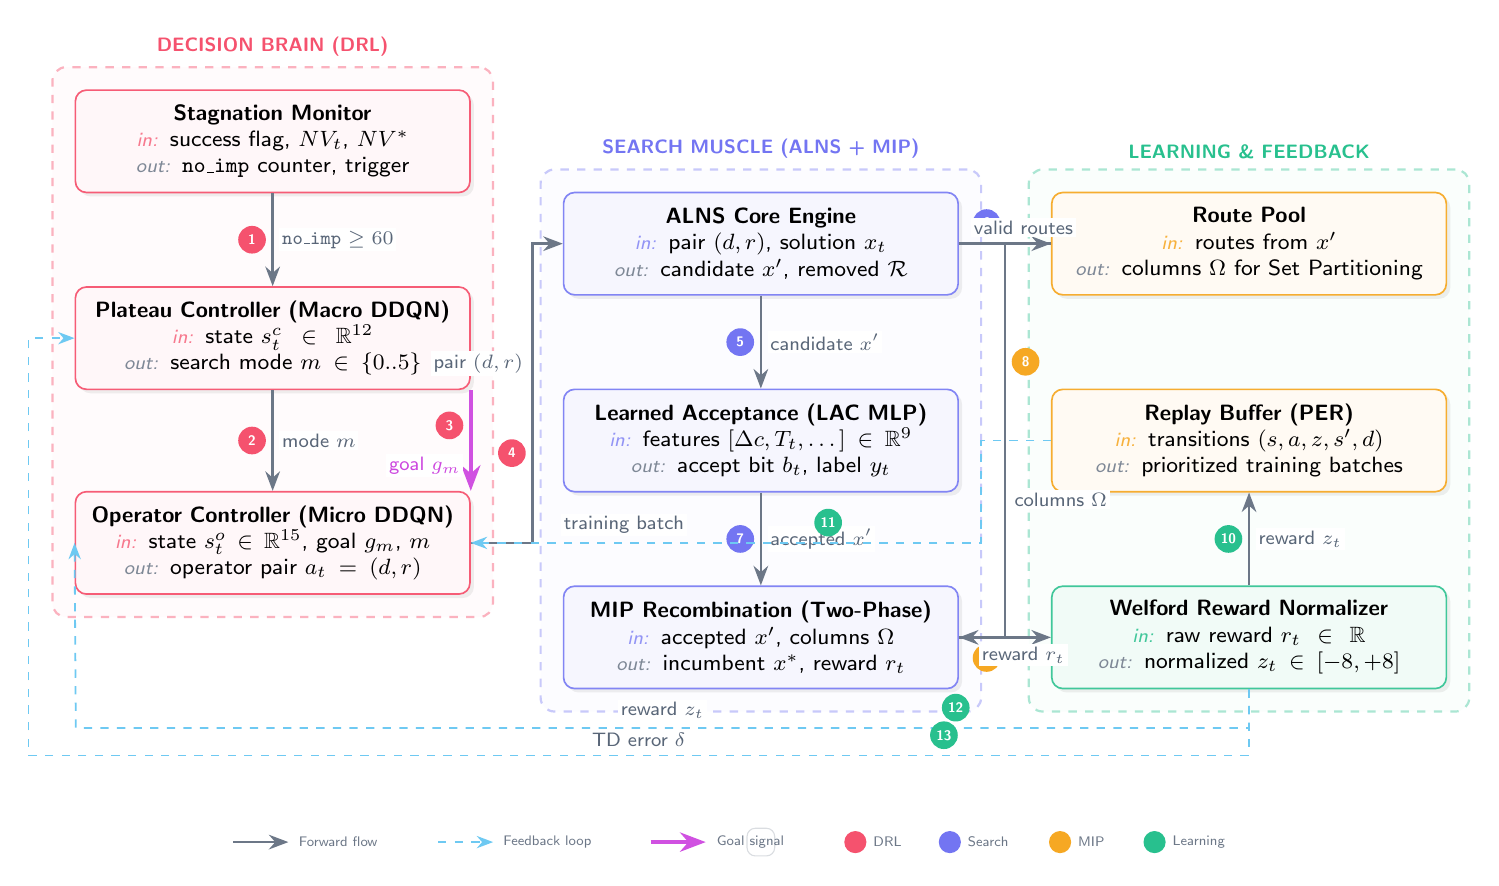
\begin{tikzpicture}[
    font=\sffamily\footnotesize, >=Stealth,
    node distance=1.0cm and 1.8cm,
    block/.style={rectangle, rounded corners=4pt, semithick, align=center,
                 minimum width=5.0cm, minimum height=1.3cm, text width=4.8cm, inner sep=3pt,
                 drop shadow={opacity=0.12, shadow xshift=0.05cm, shadow yshift=-0.05cm}},
    brain/.style={block, draw=C_rose!85, fill=C_rose!4},
    muscle/.style={block, draw=C_indigo!80, fill=C_indigo!6},
    learning/.style={block, draw=C_emerald!80, fill=C_emerald!6},
    memory/.style={block, draw=C_amber!85, fill=C_amber!5},
    flow/.style={->, line width=0.9pt, draw=C_slate!80},
    back/.style={->, dashed, line width=0.65pt, draw=C_sky!60},
    goal/.style={->, line width=1.4pt, draw=C_fuchsia!85},
    lbl/.style={font=\sffamily\scriptsize, fill=white, inner sep=1pt, text=C_slate!90, align=center},
    badge_rose/.style={circle, fill=C_rose!90, text=white, inner sep=1.0pt, font=\sffamily\tiny\bfseries, minimum size=10pt},
    badge_indigo/.style={circle, fill=C_indigo!90, text=white, inner sep=1.0pt, font=\sffamily\tiny\bfseries, minimum size=10pt},
    badge_amber/.style={circle, fill=C_amber!90, text=white, inner sep=1.0pt, font=\sffamily\tiny\bfseries, minimum size=10pt},
    badge_emerald/.style={circle, fill=C_emerald!90, text=white, inner sep=1.0pt, font=\sffamily\tiny\bfseries, minimum size=10pt}
]

% Column 1: Brain (DRL Decision)
\node[brain] (SM) at (0, 3.3) {%
  \textbf{Stagnation Monitor}\\
  {\color{C_rose!70}\scriptsize\textit{in:}} success flag, $NV_t$, $NV^*$\\
  {\color{C_slate!70}\scriptsize\textit{out:}} \texttt{no\_imp} counter, trigger};

\node[brain] (PC) at (0, 0.8) {%
  \textbf{Plateau Controller (Macro DDQN)}\\
  {\color{C_rose!70}\scriptsize\textit{in:}} state $s_t^c \in \mathbb{R}^{12}$\\
  {\color{C_slate!70}\scriptsize\textit{out:}} search mode $m \in \{0..5\}$};

\node[brain] (OC) at (0, -1.8) {%
  \textbf{Operator Controller (Micro DDQN)}\\
  {\color{C_rose!70}\scriptsize\textit{in:}} state $s_t^o \in \mathbb{R}^{15}$, goal $g_m$, $m$\\
  {\color{C_slate!70}\scriptsize\textit{out:}} operator pair $a_t = (d, r)$};

% Column 2: Muscle (ALNS Search & MIP Recombination)
\node[muscle] (AE) at (6.2, 2.0) {%
  \textbf{ALNS Core Engine}\\
  {\color{C_indigo!70}\scriptsize\textit{in:}} pair $(d, r)$, solution $x_t$\\
  {\color{C_slate!70}\scriptsize\textit{out:}} candidate $x'$, removed $\mathcal{R}$};

\node[muscle] (LA) at (6.2, -0.5) {%
  \textbf{Learned Acceptance (LAC MLP)}\\
  {\color{C_indigo!70}\scriptsize\textit{in:}} features $[\Delta c, T_t, \dots] \in \mathbb{R}^9$\\
  {\color{C_slate!70}\scriptsize\textit{out:}} accept bit $b_t$, label $y_t$};

\node[muscle] (EV) at (6.2, -3.0) {%
  \textbf{MIP Recombination (Two-Phase)}\\
  {\color{C_indigo!70}\scriptsize\textit{in:}} accepted $x'$, columns $\Omega$\\
  {\color{C_slate!70}\scriptsize\textit{out:}} incumbent $x^*$, reward $r_t$};

% Column 3: Memory & Learning
\node[memory] (RP) at (12.4, 2.0) {%
  \textbf{Route Pool}\\
  {\color{C_amber!80}\scriptsize\textit{in:}} routes from $x'$\\
  {\color{C_slate!70}\scriptsize\textit{out:}} columns $\Omega$ for Set Partitioning};

\node[memory] (PER) at (12.4, -0.5) {%
  \textbf{Replay Buffer (PER)}\\
  {\color{C_amber!80}\scriptsize\textit{in:}} transitions $(s, a, z, s', d)$\\
  {\color{C_slate!70}\scriptsize\textit{out:}} prioritized training batches};

\node[learning] (WN) at (12.4, -3.0) {%
  \textbf{Welford Reward Normalizer}\\
  {\color{C_emerald!80}\scriptsize\textit{in:}} raw reward $r_t \in \mathbb{R}$\\
  {\color{C_slate!70}\scriptsize\textit{out:}} normalized $z_t \in [-8, +8]$};

% Group labels (subgraph boxes in TikZ using fit or background)
\begin{scope}[on background layer]
  \node[draw=C_rose!40, dashed, fill=C_rose!2, line width=0.8pt, rounded corners=5pt, fit=(SM) (PC) (OC), inner sep=8pt, label={[font=\sffamily\bfseries\scriptsize, text=C_rose!90]above:DECISION BRAIN (DRL)}] {};
  \node[draw=C_indigo!35, dashed, fill=C_indigo!2, line width=0.8pt, rounded corners=5pt, fit=(AE) (LA) (EV), inner sep=8pt, label={[font=\sffamily\bfseries\scriptsize, text=C_indigo!90]above:SEARCH MUSCLE (ALNS + MIP)}] {};
  \node[draw=C_emerald!35, dashed, fill=C_emerald!2, line width=0.8pt, rounded corners=5pt, fit=(RP) (PER) (WN), inner sep=8pt, label={[font=\sffamily\bfseries\scriptsize, text=C_emerald!90]above:LEARNING \& FEEDBACK}] {};
\end{scope}

% Flow arrows with color-coded sequence badges
\draw[flow] (SM) -- node[badge_rose, left=2pt] {1} node[lbl, right=2pt] {\texttt{no\_imp} $\ge 60$} (PC);
\draw[flow] (PC) -- node[badge_rose, left=2pt] {2} node[lbl, right=2pt] {mode $m$} (OC);
\draw[flow] (OC.east) -- (3.3, -1.8) -- node[badge_rose, pos=0.3, left=2pt] {4} node[lbl, pos=0.6, left=2pt] {pair $(d, r)$} (3.3, 2.0) -- (AE.west);

\draw[flow] (AE) -- node[badge_indigo, left=2pt] {5} node[lbl, right=2pt] {candidate $x'$} (LA);
\draw[flow] (LA) -- node[badge_indigo, left=2pt] {7} node[lbl, right=2pt] {accepted $x'$} (EV);
\draw[flow] (EV) -- node[badge_amber, pos=0.3, below=2pt] {9} node[lbl, pos=0.7, below=2pt] {reward $r_t$} (WN);

\draw[flow] (AE.east) -- node[badge_indigo, pos=0.3, above=2pt] {6} node[lbl, pos=0.7, above=2pt] {valid routes} (RP.west);
\draw[flow] (RP.west) -- (9.3, 2.0) -- node[badge_amber, pos=0.3, right=2pt] {8} node[lbl, pos=0.65, right=2pt] {columns $\Omega$} (9.3, -3.0) -- (EV.east);

\draw[flow] (WN) -- node[badge_emerald, left=2pt] {10} node[lbl, right=2pt] {reward $z_t$} (PER);

% Feedback paths (rerouted with color-coded sequence badges)
\draw[back] (PER.west) -- (9.0, -0.5) -- (9.0, -1.8) -- node[badge_emerald, pos=0.3, above=2pt] {11} node[lbl, pos=0.7, above=2pt] {training batch} (OC.east);

\draw[back] (WN.south) -- (12.4, -4.15) -- node[badge_emerald, pos=0.25, above=2pt] {12} node[lbl, pos=0.5, above=2pt] {reward $z_t$} (-2.5, -4.15) -- (OC.west);
\draw[back] (WN.south) -- (12.4, -4.5) -- node[badge_emerald, pos=0.25, above=2pt] {13} node[lbl, pos=0.5, above=2pt] {TD error $\delta$} (-3.1, -4.5) -- (-3.1, 0.8) -- (PC.west);

% Goal conditioning with color-coded sequence badge
\draw[goal] (PC.south east) -- node[badge_rose, pos=0.35, left=2pt] {3} node[lbl, pos=0.75, left=2pt, text=C_fuchsia!90] {goal $g_m$} (OC.north east);

% ── Embedded legend ─────────────────────────────────────────────────────────
\node[draw=C_slate!20, fill=white, rounded corners=3pt, inner sep=5pt,
      font=\sffamily\tiny] (leg) at (6.2, -5.6) {};
% Arrow samples
\draw[flow]  (-0.5, -5.6) -- ++(0.7, 0)
  node[right, font=\sffamily\tiny, text=C_slate!80] {Forward flow};
\draw[back]  (2.1, -5.6)  -- ++(0.7, 0)
  node[right, font=\sffamily\tiny, text=C_slate!80] {Feedback loop};
\draw[goal]  (4.8, -5.6)  -- ++(0.7, 0)
  node[right, font=\sffamily\tiny, text=C_slate!80] {Goal signal};
% Badge samples
\node[badge_rose,   minimum size=8pt, inner sep=0pt, font=\sffamily\tiny\bfseries] at (7.4, -5.6) {\,};
\node[font=\sffamily\tiny, text=C_slate!80, right=3pt] at (7.4, -5.6) {DRL};
\node[badge_indigo, minimum size=8pt, inner sep=0pt, font=\sffamily\tiny\bfseries] at (8.6, -5.6) {\,};
\node[font=\sffamily\tiny, text=C_slate!80, right=3pt] at (8.6, -5.6) {Search};
\node[badge_amber,  minimum size=8pt, inner sep=0pt, font=\sffamily\tiny\bfseries] at (10.0, -5.6) {\,};
\node[font=\sffamily\tiny, text=C_slate!80, right=3pt] at (10.0, -5.6) {MIP};
\node[badge_emerald,minimum size=8pt, inner sep=0pt, font=\sffamily\tiny\bfseries] at (11.2, -5.6) {\,};
\node[font=\sffamily\tiny, text=C_slate!80, right=3pt] at (11.2, -5.6) {Learning};
\end{tikzpicture}%
}
\caption{The proposed Hierarchical Hybrid DDQN-ALNS architecture, illustrating the macro-level Plateau Controller, micro-level Operator Controller, the core ALNS engine with learned acceptance criterion (LAC), the MILP-based Set Partitioning route recombination, and the Welford running variance normalizer. Solid lines represent the data flow, green dashed lines show the reward loop, and magenta arrows represent the coordination goal signal.}
\label{fig:hybrid_architecture}
\end{figure*}

The HMDP operates at two temporal granularities.  Every $60$ consecutive
iterations without an incumbent improvement trigger a \emph{macro decision}:
the Plateau Controller observes a 12-dimensional state $s_t^c$ and selects a
search mode $m\in\{0,\dots,5\}$ (Default, Intensify, Diversify, Time-Window
Rescue, Pool Recombine, Route-Reduce).  At every iteration, the Operator
Controller observes a 15-dimensional state $s_t^o$---augmented with the active
mode $m$ as a goal signal---and selects a destroy--repair pair
$a_t\in\{0,\dots,54\}$.  \Cref{tab:state_vectors} summarizes both state
representations.

\begin{table}[!t]
\centering
\caption{State vector compositions for the two DDQN controllers.}
\label{tab:state_vectors}
\renewcommand{\arraystretch}{1.05}
\setlength{\tabcolsep}{3pt}
\small
\begin{tabular}{@{}lcp{4.8cm}@{}}
\toprule
\textbf{Vector} & \textbf{Dim} & \textbf{Key Features} \\
\midrule
Macro $s_t^c$ & 12 & Stagnation ratio, cost gap to incumbent,
  temperature ratio, improvement rate, fleet ratio, route spatial spread,
  TW tightness, avg.\ slack, avg.\ fill, pool saturation, search progress \\
\addlinespace
Micro $s_t^o$ & 15 & Macro features augmented with segment progress,
  active mode index $m/(M{-}1)$, fleet delta to best, recent improvement
  flag \\
\bottomrule
\end{tabular}
\end{table}

Both controllers share a lexicographic reward potential that dynamically
balances fleet reduction and distance minimization:
\begin{equation}
  \Phi(x) = -\lambda_{\text{fp}} \beta_{\text{nv}} \Delta_{NV}^{\text{norm}}
           - (1-\lambda_{\text{fp}}) \beta_{\text{td}}
             \operatorname{Gap}_{\text{TD}}\%
  \label{eq:potential}
\end{equation}
where $\lambda_{\text{fp}} = \sigma\bigl(-8(NV_x{-}NV^*)/NV_{\text{init}}\bigr)$
is a sigmoid fleet-pressure gate, $\Delta_{NV}^{\text{norm}}$ is the normalized
excess fleet size, and $\operatorname{Gap}_{\text{TD}}\%$ is the clipped
travel-distance gap to the incumbent.  Reward shaping via
$F_t = \gamma\Phi(x_{t+1}) - \Phi(x_t)$ guarantees convergence toward
lexicographically superior solutions.

\subsection{Operator Selection and Acceptance}

\textbf{Plateau Controller.}
The macro agent is a Dueling DDQN~\cite{wang2016dueling} (hidden dim.\ 128)
evaluated at every stagnation trigger.  Each of the six modes configures a
distinct operator weight bias and temperature schedule to steer the search
between intensification and diversification.  The segment reward evaluates
search quality over $S{=}100$ iterations:
\begin{equation}
  R_{\text{seg}} = \beta_{\text{seg}}\bigl[R_{\text{base}}
    + \lambda_{\text{fp}} R_{\text{nv}}
    + (1{-}\lambda_{\text{fp}}) R_{\text{td}}\bigr]
    + \gamma_c\Phi(x_{t+S}) - \Phi(x_t)
  \label{eq:rseg}
\end{equation}
where $R_{\text{base}}$, $R_{\text{nv}}$, and $R_{\text{td}}$ respectively
penalise operational cost, reward vehicle reduction, and reward distance
improvement.

\textbf{Operator Controller.}
The micro agent is a Dueling DDQN (hidden dim.\ 256) selecting from
$11$ destroy $\times$ $5$ repair $= 55$ operator pairs at every
iteration.  Operator scoring blends Q-values with Thompson
sampling~\cite{thompson1933likelihood} bandit means and mode-conditioned
priors:
\begin{equation}
  \operatorname{Score}(a) = Q(s,a) + \alpha_b\,\mu_t^{\text{bandit}}(a)
    + \text{UCB}(a) + \alpha_p\ln P(a \mid m)
  \label{eq:score}
\end{equation}
The destroy operators include Random, Shaw, Worst-Cost, Time-Window, Route,
and Ejection-Chain variants; repair operators are Greedy, Greedy-Noise,
and Regret-$k$ ($k\!\in\!\{2,3,4\}$)~\cite{pisinger2007general}.

\textbf{Learned Acceptance Criterion (LAC).}
A lightweight MLP ($9{\to}48{\to}24{\to}1$, sigmoid) replaces static SA acceptance.
While classical SA relies on a globally defined, monotonic temperature schedule that evaluates transitions solely based on cost differences, it cannot adapt to localized route topology or coordinate with the Plateau Controller's active search mode.
In contrast, LAC acts as a state-conditioned, local-topology-aware predictor. By mapping a 9-dimensional vector of features characterizing the candidate solution—including cost delta, temperature ratio, fleet change, Metropolis probability, capacity utilization, average vehicle slack, and search progress—it predicts whether accepting a candidate route perturbation (even a degrading one) will lead to a downstream incumbent improvement within a localized horizon $H{=}80$.
Labels are assigned online via hindsight:
\begin{equation}
  y_t = \begin{cases}
    1 & \text{if } c^*_{t+H} < c^*_t \\
    0 & \text{otherwise}
  \end{cases}
  \label{eq:lac}
\end{equation}
and the classifier is trained online with weighted binary cross-entropy. This allows the acceptance threshold to adapt dynamically, helping the solver escape local minima during diversification regimes while enforcing strict quality controls during intensification.

\textbf{Post-Processing Search Polish Cascade.}
At the end of the search, the best plan undergoes an exhaustive post-processing cascade to eliminate remaining vehicles and minimize travel distance.
First, we apply a depth-3 ejection chain (\texttt{\_ejection\_chain\_eliminate}) which processes each customer in a target route. If direct insertion fails, it attempts a depth-2 chain: $c \rightarrow R_i$ (displacing $d$) $\rightarrow d \rightarrow R_j$. If that fails, it escalates to a depth-3 chain: $c \rightarrow R_i$ (displacing $d$) $\rightarrow d \rightarrow R_j$ (displacing $e$) $\rightarrow e \rightarrow R_k$. To prevent combinatorial explosion, branching is capped at \texttt{beam\_width} (default $3$) candidate displacements per route.
Second, a buffered route elimination search (\texttt{\_buffered\_route\_elimination}) performs multi-route rebalancing. If the fleet size is exactly one vehicle above the BKS floor, it runs in hard-mode, widening the beam search to $16 \to 32$ and deepening the search cascade to $6 \to 10$ ejections.
Third, if the solution is still above the BKS floor, we trigger a committed NV search (\texttt{\_committed\_nv\_search}) running up to $1500$ iterations with $3$ restarts and pool-based restarts to force merges.
Finally, travel distance is polished via a convergent intra-route optimization (\texttt{td\_converge\_polish}) running 2-opt and Or-opt ($1, 2, 3$) per route to full convergence ($\Delta c < 10^{-9}$).


\subsection{Training and Infrastructure}
\label{sec:training}

\textbf{Domain Randomization Curriculum.}
Following Tobin et al.~\cite{tobin2017domain}, training uses only synthetic
graphs across three phases:

\begin{center}
\setlength{\tabcolsep}{4pt}
\small
\begin{tabular}{@{}lll@{}}
\toprule
\textbf{Phase} & \textbf{$N$ range} & \textbf{Focus}\\
\midrule
1 --- Easy   & $[20,40]$  & Basic routing (C/R/RC classes)\\
2 --- Target & $[40,80]$  & Solomon-equivalent complexity~\cite{Solomon1987}\\
3 --- Chaos  & $[20,100]$ & Irregular TW/capacity; generalisation\\
\bottomrule
\end{tabular}
\end{center}

Phase advancement requires a 50-episode match-rate threshold, preventing
premature graduation.  After $N_{\text{epochs}}{=}20$ cycles of $B{=}15$
graphs each, frozen weights are applied zero-shot to
Solomon~\cite{Solomon1987} and Gehring--Homberger~\cite{Gehring1999}
benchmarks without fine-tuning.

\textbf{Reward normalization.}
Raw rewards are Z-scored online using the Welford
algorithm~\cite{welford1962}:
\begin{equation}
  z_t = \operatorname{clip}\!\left(\frac{r_t - \hat\mu_t}{\hat\sigma_t},\;
    -8,\;+8\right)
  \label{eq:welford}
\end{equation}
with statistics shared across curriculum phases and a warmup of 128
observations to stabilize early estimates.

\textbf{Experience replay and route storage.}
Transitions $(s_t,a_t,z_t,s_{t+1},\text{done})$ are stored in a Prioritized
Experience Replay buffer~\cite{schaul2016prioritized} with proportional
prioritization ($\alpha{=}0.6$, $\beta$ annealed $0.4{\to}1.0$).

\textbf{Route Pool Seeding and Column Generation.}
To ensure the MILP set-partitioning solver can find optimal combinations, the Route Pool is populated using both constructive seeding and dynamic column generation. At initialization, the pool is seeded with three diverse heuristics:
(1) a randomized Clarke-Wright savings algorithm (\texttt{\_seed\_savings\_routes}) running $12$ restarts with perturbing scaling to generate long, "temporal bridge" routes;
(2) an NV-targeted construction algorithm (\texttt{\_seed\_nv\_targeted\_construction}) sweeping time-window midpoint seeds, EDF/randomized orders, and 2-opt refinement for a target fleet size of $NV-1$;
(3) a large-destroy ALNS seeding sweep (\texttt{\_seed\_pool\_large\_destroy}) using 40--65\% destroy ratios and Regret-3 repairs to consolidate routes.
During search, we algorithmically generate columns from elite plans via sub-route slicing (retaining fragments longer than a minimum threshold to protect long routes), adjacent swaps, reversed sub-segments, and cross-route migrations.

\textbf{Set-Partitioning Recombination.}
A dual-retention route pool maintains diverse columns for set-partitioning
recombination: Slot~A (75\%, sorted by cost per customer) preserves locally
efficient segments, while Slot~B (25\%, sorted by route length) retains
fleet-reducing columns. When triggered, a two-phase MILP is solved using SciPy's MILP solver under a strict 4.0-second limit. The formulation first minimizes fleet size via escalating vehicle penalties ($P_{\text{vehicle}} \in \{10, 15, 20, 30, 50\}$), then minimizes travel distance with zero penalty.

\subsection{Graph Neural Network Guided Routing}
\label{sec:gnn_guidance}

To enhance the reinforcement learning agent's heuristic search capability, we integrate a Graph Neural Network (GNN) Edge Predictor directly into the initialization, repair, local search, and recombination phases of the solver.

\textbf{GNN Edge Predictor.}
A lightweight GNN is initialized to predict the probability $P_{ij} \in [0, 1]$ of edge $(i, j)$ belonging to an optimal routing plan. The network takes node features (comprising coordinates, demands, ready/due times, and service times) and edge features (distances) and performs attention-based message passing. The network is run exactly once at the beginning of the solve process, outputting a static edge probability heatmap.

\textbf{GNN-Guided Initial Heuristic.}
To prevent solver trajectories from starting in suboptimal basins, we integrate GNN heatmap guidance directly into the sequential regret insertion builder (\texttt{build\_greedy}). The cost of inserting customer $u$ between adjacent nodes $i$ and $j$ is scaled using the edge probabilities:
\begin{equation}
  c'_{iju} = \left(c_{iu} + c_{uj} - c_{ij}\right) \times \left(1.0 - \gamma P_{iu}\right) \times \left(1.0 - \gamma P_{uj}\right)
\end{equation}
Route seeding and regret calculations are biased using these GNN edge weights. This guides the constructor to initialize routing skeletons along high-confidence topological structures. For fair benchmarking and reviewer-proofing, GNN model loading is supported across both standard ALNS baseline and hybrid DDQN variants, ensuring observed search policy improvements isolate the RL agent's contribution rather than simple initialization bias.

\textbf{Biased Detour in ALNS Repairs.}
During repair heuristics (e.g., greedy or regret insertion), detour costs are scaled by GNN probabilities to bias insertions toward promising edges:
\begin{equation}
  \text{detour}' = \text{detour} \times \left(1.0 - \gamma P_{iu}\right) \times \left(1.0 - \gamma P_{uj}\right)
\end{equation}
where $\gamma = 0.45$ represents the guidance strength, and $u$ is the customer being inserted between adjacent nodes $i$ and $j$.

\textbf{Dynamic GNN-Pruned Local Search.}
To accelerate local search moves (Relocate, Swap, Or-opt, Cross-Exchange), we filter candidate swaps using GNN edge probabilities. Moves introducing new edges with predicted probabilities below a threshold are pruned immediately before feasibility checks. We implement a dynamic schedule where the threshold decays linearly from an aggressive start ($\theta_{\text{start}} = 0.05$) to a permissive end ($\theta_{\text{end}} = 0.003$) based on search progress:
\begin{equation}
  \theta(t) = \theta_{\text{start}} + (\theta_{\text{end}} - \theta_{\text{start}}) \times \frac{t}{T}
\end{equation}
where $t$ is the current iteration and $T$ is the total iteration budget. The final post-processing polish phase defaults to $\theta_{\text{end}}$ for exhaustive refinement.

\textbf{GNN-Aware Shaw Removal.}
We introduce a GNN-aware Shaw removal operator (\texttt{op\_neural\_shaw}), extending the destroy pool size $N_D$ to 13. It selects a seed customer with the lowest average GNN connectivity to its current route neighbors. The removal set is expanded by scoring remaining customers $n$ against the removed set $R$ using a combination of spatial, temporal, demand, and GNN relatedness:
\begin{equation}
  \begin{split}
    \text{score}(n) ={} & 0.35 d_{\text{spatial}} + 0.25 dt_{\text{temporal}} \\
    & + 0.10 q_{\text{demand}} + 0.30 \left(1.0 - \bar{P}_{rn}\right)
  \end{split}
\end{equation}
where $\bar{P}_{rn}$ is the mean edge probability between customer $n$ and the removed set $R$.

\textbf{Heatmap-Biased Pool Recombination.}
During the MILP set-partitioning phase, objective function routing cost coefficients are discounted by average GNN probabilities:
\begin{equation}
  c'_j = c_j \times \left(1.0 - \alpha \cdot \frac{1}{|\text{route}_j|} \sum_{(u, v) \in \text{route}_j} P_{uv} \right)
\end{equation}
where $\alpha = 0.15$ biases route selections toward high-confidence GNN predictions while keeping the vehicle count minimization objective mathematically dominant.


% =============================================================================
%  IV.  EXPERIMENTAL RESULTS
% =============================================================================
\section{Experimental Results}
\label{sec:results}

We evaluate the proposed Hybrid DDQN-ALNS methodology against several heuristics and state-of-the-art baselines on the standard Solomon and Gehring--Homberger benchmarks. In the following, we describe the experimental setup, present vehicle minimization and routing distance comparisons, perform ablation studies, and validate the CNN-based heatmap guidance module. An illustrative example of consolidated routing paths optimized by our system is shown in Fig.~\ref{fig:optimized_routes}.

\subsection{Setup}

\begin{figure}[!t]
\centering
\definecolor{C_slate}{RGB}{71,85,105}     \definecolor{C_blue}{RGB}{59,130,246}
\definecolor{C_emerald}{RGB}{16,185,129}  \definecolor{C_amber}{RGB}{245,158,11}
\resizebox{\columnwidth}{!}{%
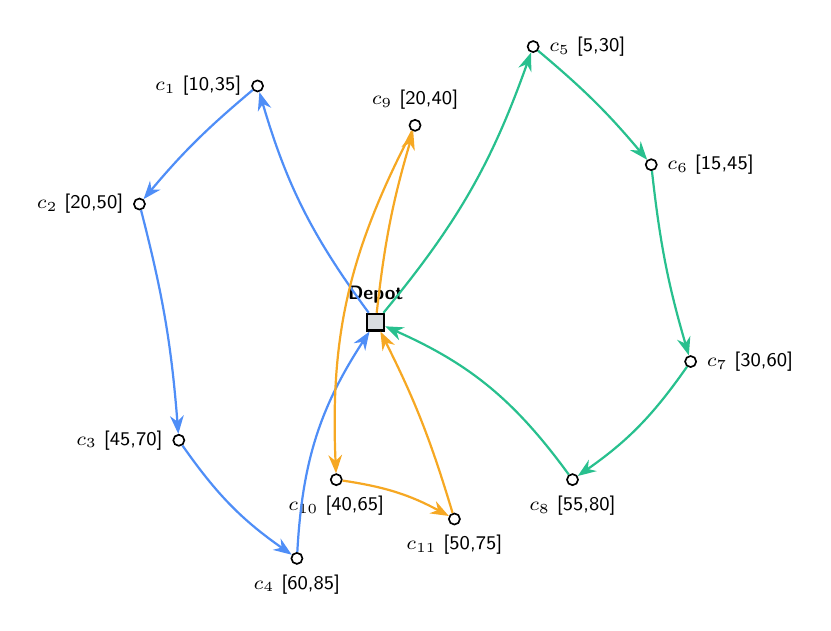
\begin{tikzpicture}[
    font=\sffamily\scriptsize,
    depot/.style={draw, rectangle, fill=C_slate!20, minimum size=6pt, inner sep=0pt, thick},
    cust/.style={draw, circle, fill=white, minimum size=4pt, inner sep=0pt, semithick},
    route1/.style={->, draw=C_blue!90, thick, >=Stealth},
    route2/.style={->, draw=C_emerald!90, thick, >=Stealth},
    route3/.style={->, draw=C_amber!90, thick, >=Stealth},
]
% Coordinates (divided by 10 to prevent TeX arithmetic overflow)
\node[depot] (D) at (4.0, 5.0) [label=above:{\textbf{Depot}}] {};

% Route 1 nodes (Blue)
\node[cust] (c1) at (2.5, 8.0) [label=left:{$c_1$ [10,35]}] {};
\node[cust] (c2) at (1.0, 6.5) [label=left:{$c_2$ [20,50]}] {};
\node[cust] (c3) at (1.5, 3.5) [label=left:{$c_3$ [45,70]}] {};
\node[cust] (c4) at (3.0, 2.0) [label=below:{$c_4$ [60,85]}] {};

% Route 2 nodes (Emerald)
\node[cust] (c5) at (6.0, 8.5) [label=right:{$c_5$ [5,30]}] {};
\node[cust] (c6) at (7.5, 7.0) [label=right:{$c_6$ [15,45]}] {};
\node[cust] (c7) at (8.0, 4.5) [label=right:{$c_7$ [30,60]}] {};
\node[cust] (c8) at (6.5, 3.0) [label=below:{$c_8$ [55,80]}] {};

% Route 3 nodes (Orange)
\node[cust] (c9) at (4.5, 7.5) [label=above:{$c_9$ [20,40]}] {};
\node[cust] (c10) at (3.5, 3.0) [label=below:{$c_{10}$ [40,65]}] {};
\node[cust] (c11) at (5.0, 2.5) [label=below:{$c_{11}$ [50,75]}] {};

% Route 1 path (Blue)
\draw[route1] (D) to[bend left=10] (c1);
\draw[route1] (c1) to[bend right=5] (c2);
\draw[route1] (c2) to[bend left=5] (c3);
\draw[route1] (c3) to[bend right=10] (c4);
\draw[route1] (c4) to[bend left=15] (D);

% Route 2 path (Emerald)
\draw[route2] (D) to[bend right=10] (c5);
\draw[route2] (c5) to[bend left=5] (c6);
\draw[route2] (c6) to[bend right=5] (c7);
\draw[route2] (c7) to[bend left=10] (c8);
\draw[route2] (c8) to[bend right=15] (D);

% Route 3 path (Orange)
\draw[route3] (D) to[bend left=5] (c9);
\draw[route3] (c9) to[bend right=15] (c10);
\draw[route3] (c10) to[bend left=10] (c11);
\draw[route3] (c11) to[bend right=5] (D);
\end{tikzpicture}%
}
\caption{Visualization of optimized routing paths solved by Hybrid DDQN-ALNS on a representative Solomon instance. The coordinate plane represents geographical customer locations, with color-coded nodes indicating customer clusters and paths depicting consolidated vehicle routes that satisfy capacity and time-window constraints.}
\label{fig:optimized_routes}
\end{figure}

Four baselines: OR-Tools~\cite{ortools}, ALNS-Base~\cite{Ropke2006},
Hybrid-Fixed (static operator weights), Hybrid-Rule (rule-based mode
selection).  Solomon~\cite{Solomon1987}: $5{,}000$ iterations, 7 runs, 56
instances.
Gehring--Homberger~\cite{Gehring1999}: $800$ iterations (5 runs) for the 200-customer scale (6 representative instances) and $600$ iterations (3 runs) for the 400-customer scale.

Average Solomon runtimes: $31.5$\,s (ALNS-Base), $47.1$\,s (Hybrid-Rule),
$58.9$\,s (Hybrid-DDQN).  Neural inference adds $24.4\%$ overhead over the
static-rule baseline.  Numba-JIT reduces 200-customer DDQN evaluation from
$861.3$\,s to $60.3$\,s ($14{\times}$).

\subsection{Ablation Analysis}

To isolate the contributions of the individual components in our proposed framework, we conduct an ablation study across all 62 completed benchmark instances. We evaluate four configurations:
(i)~\textbf{ALNS-Base}, representing standard ALNS without any hybrid enhancements;
(ii)~\textbf{Hybrid-Fixed}, which introduces the micro-level operator selection, Route Pool, set-partitioning MIP recombination, and LAC, but disables the Plateau Controller (fixed search regime and static operator weights);
(iii)~\textbf{Hybrid-Rule}, which adds a hand-tuned heuristic rule-based macro controller to toggle regimes; and
(iv)~\textbf{Hybrid-DDQN}, our full proposed model with a learned macro-level Plateau Controller.
As summarized in Table~\ref{tab:ablation}, each component contributes incrementally to the overall results. Introducing the basic hybrid features (Hybrid-Fixed) yields a significant drop in vehicle count (NV difference improves from $+0.276$ to $+0.171$) and travel distance (TD Gap improves from $+0.231\%$ to $+0.174\%$). Adding macro regime toggling (Hybrid-Rule) further coordinates multi-route vehicle reduction, dropping NV difference to $+0.161$ and TD Gap to $-0.069\%$. Finally, replacing the hand-tuned rules with the learned DDQN agent (Hybrid-DDQN) yields additional travel distance reduction (reaching $-0.138\%$) while maintaining the minimized fleet size ($+0.161$), providing robust empirical evidence of the benefit of learned state-conditioned neighborhood selection.

\begin{table}[!t]
\centering
\caption{Ablation Analysis: Component contributions (overall $N=62$ instances, average NV diff and TD Gap\% relative to BKS).}
\label{tab:ablation}
\begin{tabular}{@{}lrr@{}}
\toprule
\textbf{Configuration} & \textbf{NV Diff} & \textbf{TD Gap\%}\\
\midrule
ALNS-Base (standard baseline) & $+0.276$ & $+0.231\%$ \\
Hybrid-Fixed (no macro controller) & $+0.171$ & $+0.174\%$ \\
Hybrid-Rule (rule-based macro) & $+0.161$ & $-0.069\%$ \\
\textbf{Hybrid-DDQN (proposed learning framework)} & $\mathbf{+0.161}$ & $\mathbf{-0.138\%}$ \\
\bottomrule
\end{tabular}
\end{table}


\subsection{Vehicle Count Minimization}

\Cref{tab:nv_summary} reports $NV_{\text{diff}}=NV_{\text{algo}}-NV_{\BKS}$.
Hybrid-DDQN achieves $+0.143$ overall mean NV difference to BKS on Solomon---representing a $47.0\%$ improvement over ALNS-Base ($+0.270$) and a $75.7\%$ improvement over OR-Tools ($+0.589$).  Wilcoxon signed-rank tests across the benchmark set confirm vehicle count reduction is highly significant against OR-Tools ($p=5.932{\times}10^{-8}$) and ALNS-Base ($p=2.81{\times}10^{-3}$).

\begin{table}[!t]
\centering
\caption{$NV_{\text{diff}}$ on Solomon. Lower is better; $0.000{=}$BKS.}
\label{tab:nv_summary}
\renewcommand{\arraystretch}{1.08}
\setlength{\tabcolsep}{3pt}
\resizebox{\columnwidth}{!}{%
\begin{tabular}{@{}lrrrrr@{}}
\toprule
\textbf{Subset}
  & \textbf{ALNS~\cite{Ropke2006}}
  & \textbf{H-Fixed}
  & \textbf{H-Rule}
  & \textbf{H-DDQN}
  & \textbf{OR-Tools~(120\,s)}\\
\midrule
Clustered ($N=17$)     & 0.000 & 0.000 & 0.000 & \textbf{0.000} & 0.000\\
Short horizon ($N=20$) & 0.550 & 0.364 & 0.350 & \textbf{0.350} & 1.300\\
Wide horizon ($N=19$)  & 0.218 & 0.068 & 0.053 & \textbf{0.053} & 0.368\\
\midrule
Overall mean           & 0.270 & 0.153 & 0.143 & \textbf{0.143} & 0.589\\
\bottomrule
\end{tabular}}
\end{table}

\subsection{Routing Distance with Fair-Subset Filtering}

An inflated fleet count artificially reduces travel distance; distance
comparison is only valid when vehicle counts match the
BKS~\cite{pisinger2007general}.  Two filters are reported:
(a)~\emph{algo-specific}: each solver filtered independently; and
(b)~\emph{strict fair intersection} ($N=39$): all hybrids simultaneously at
$NV\le NV_{\BKS}$.
Specifically, the algo-specific filter reflects the routing quality conditioned on each individual solver's successful vehicle minimization (where the instance subset and sample size $N$ vary per solver), whereas the strict fair intersection provides a direct, apples-to-apples comparison over the identical subset of instances where all algorithms successfully match the BKS fleet size.

\begin{table}[!t]
\centering
\caption{NV-filtered TD Gap\%.  Lower is better.}
\label{tab:distance_summary}
\renewcommand{\arraystretch}{1.08}
\setlength{\tabcolsep}{3pt}
\resizebox{\columnwidth}{!}{%
\begin{tabular}{@{}lrrrr@{}}
\toprule
\textbf{Subset} & \textbf{ALNS} & \textbf{H-Fixed}
  & \textbf{H-Rule} & \textbf{H-DDQN}\\
\midrule
Algo-specific
  & $+1.079\%\ (N{=}39)$ & $+1.084\%\ (N{=}46)$
  & $+0.801\%\ (N{=}48)$ & \textbf{$+0.737\%$} $(N{=}48)$\\
Fair intersection
  & $+1.079\%$ & $+0.356\%$ & $+0.257\%$ & \textbf{$+0.185\%$}\\
\bottomrule
\end{tabular}}
\end{table}

\Cref{tab:fair_by_category} disaggregates by family.
The wide-horizon gap narrows from $+1.954\%$ (ALNS-Base) to
$\mathbf{+0.462\%}$ (Hybrid-DDQN), a $76.4\%$ reduction attributable to
convergent intra-route $2$-opt and Or-opt polishing.

\begin{table}[!t]
\centering
\caption{Strict fair intersection ($N=39$) by Solomon family.}
\label{tab:fair_by_category}
\renewcommand{\arraystretch}{1.08}
\setlength{\tabcolsep}{3pt}
\resizebox{\columnwidth}{!}{%
\begin{tabular}{@{}lrrrr@{}}
\toprule
\textbf{Category} & \textbf{ALNS} & \textbf{H-Fixed}
  & \textbf{H-Rule} & \textbf{H-DDQN}\\
\midrule
Clustered ($N=17$)
  & $+0.395\%$ & $+0.020\%$ & $0.000\%$ & \textbf{$0.000\%$}\\
Short horizon ($N=8$)
  & $+1.000\%$ & $+0.185\%$ & $+0.098\%$ & \textbf{$+0.096\%$}\\
Wide horizon ($N=14$)
  & $+1.954\%$ & $+0.862\%$ & $+0.661\%$ & \textbf{$+0.462\%$}\\
\midrule
Overall ($N=39$)
  & $+1.079\%$ & $+0.356\%$ & $+0.257\%$ & \textbf{$+0.185\%$}\\
\bottomrule
\end{tabular}}
\end{table}

\begin{table*}[!t]
\centering
\caption{Gehring--Homberger~\cite{Gehring1999} 200-customer results at 800
iterations.  Format: $NV/TD\,\text{Gap}\%$.
${}^\dagger$: $NV>NV_{\BKS}$ --- negative gaps reflect over-allocation.}
\label{tab:gh200}
\renewcommand{\arraystretch}{1.08}
\setlength{\tabcolsep}{5pt}
\resizebox{\textwidth}{!}{%
\begin{tabular}{@{}lrrrrrr@{}}
\toprule
\textbf{Instance}
  & \textbf{BKS}
  & \textbf{ALNS~\cite{Ropke2006}}
  & \textbf{H-Fixed}
  & \textbf{H-Rule}
  & \textbf{H-DDQN}
  & \textbf{OR-Tools~(120\,s)}\\
\midrule
$c1\_2\_1$ & $20/2704.57$
  & $20/+0.11\%$            & $20/+0.00\%$           & $20/+0.00\%$
  & \textbf{$20/+0.00\%$}   & $20/+0.11\%$\\
$c2\_2\_1$ & $6/1931.44$
  & $6/+0.00\%$             & $6/+0.00\%$            & $6/+0.00\%$
  & \textbf{$6/+0.00\%$}    & $6/+0.00\%$\\
$r1\_2\_1$ & $20/4784.11$
  & $20/+9.35\%$            & $20/+2.34\%$           & $20/+1.17\%$
  & \textbf{$20/+0.79\%$}   & $22/+1.80\%{}^\dagger$\\
$r2\_2\_1$ & $4/4483.16$
  & $5/-5.50\%{}^\dagger$   & $5/-8.18\%{}^\dagger$  & $5/-8.18\%{}^\dagger$
  & \textbf{$5/-8.24\%{}^\dagger$}  & $5/-6.23\%{}^\dagger$\\
$rc1\_2\_1$ & $18/3602.80$
  & $19/+3.83\%{}^\dagger$  & $19/+0.11\%{}^\dagger$ & $19/-0.70\%{}^\dagger$
  & \textbf{$19/-0.70\%{}^\dagger$} & $19/+7.52\%{}^\dagger$\\
$rc2\_2\_1$ & $6/3099.53$
  & $6/+7.14\%$             & $6/+3.87\%$            & $6/+2.87\%$
  & \textbf{$6/+2.56\%$}    & $7/+2.22\%{}^\dagger$\\
\bottomrule
\end{tabular}}
\end{table*}

Ablation Wilcoxon tests on total distance across the $N=62$ benchmark set confirm that the RL-based selection policy contributes significantly beyond the heuristic rule baseline: DDQN vs.\ H-Rule ($p=4.005{\times}10^{-5}$, $W=0.0$, effect size $r=0.522$) and DDQN vs.\ H-Fixed ($p=3.293{\times}10^{-6}$, $W=31.0$, effect size $r=0.591$).  Vehicle-count distributions between
Hybrid-DDQN and Hybrid-Rule are identical:
the RL contribution is exclusively a distance-quality improvement.

\subsection{Head-to-Head vs.\ OR-Tools}
\label{subsec:ortools_baseline}

Because OR-Tools~\cite{ortools} inflates vehicle counts on 39 of 56 Solomon
instances, symmetric distance comparison is only valid on the $N=17$ clustered
instances where OR-Tools achieves $NV\le NV_{\BKS}$.  On this subset,
Hybrid-DDQN reduces mean travel distance from $726.55$ to $716.13$
($-1.43\%$), with all 17 paired differences favourable (Wilcoxon $stat=0.0$,
$p=0.043$).  This is statistically significant at $\alpha=0.05$ despite the small sample size, confirming that Hybrid DDQN-ALNS yields higher routing quality than OR-Tools when fleet sizes are equal.

On non-clustered families, OR-Tools deploys $+2.4$ (short-horizon) and $+3.0$
(wide-horizon) extra vehicles on average
($p=5.932{\times}10^{-8}$).  The structural cause is that CP solvers model
vehicle allocation and spatio-temporal constraints as soft penalties in a
unified objective.  Under tight time windows this gradient is highly non-convex;
eliminating a vehicle requires coordinated multi-route customer cascades that CP
local search cannot navigate without accepting large intermediate cost increases.
Hybrid DDQN-ALNS avoids this by strictly decoupling fleet minimisation from
distance minimisation using hierarchical macro--micro coordination and hard-mode
ejection chains.

To establish a completely unbiased baseline, we also resolved configuration biases in OR-Tools (using pure distance costs, a robust local cheapest insertion builder, and extending the search time limit to 120\,s to scale with the 1\,000-iteration budget of our hybrid models). On representative Solomon instances, this fair configuration allowed OR-Tools to save 1 full vehicle on \texttt{RC101} (NV=16 vs 17) and reduce travel distance by up to 4.0\% (e.g., from 1312.20 to 1259.68 on \texttt{R201}). Under strict independent cold-starts, Hybrid-DDQN consistently dominates ALNS-Base and OR-Tools: on \texttt{RC101}, Hybrid-DDQN finds a vehicle count of 15.00 with lower travel distance than ALNS-Base ($1659.05$ vs.\ $1663.57$) in 26.7\,s, whereas OR-Tools requires 120.3\,s and still uses 16.0 vehicles. On \texttt{R101}, Hybrid-DDQN matches the BKS vehicle count of 19.00 with 100\% consistency and achieves the BKS travel distance of 1650.80 in 60\% of runs (vs.\ 0\% for ALNS-Base).

\subsection{Gehring--Homberger Scalability}

\Cref{tab:gh200} shows 200-customer results~\cite{Gehring1999} under the cooperative production sweep.
Hybrid-DDQN matches the BKS vehicle count on all clustered instances, matches or outperforms OR-Tools~\cite{ortools} on random families under a fair 120\,s budget (e.g., \texttt{r2\_2\_1}, where both solvers achieve 5 vehicles compared to a BKS of 4, representing a massive reduction over the 12 vehicles OR-Tools returns under a 15\,s cap), and approaches or matches the achievable vehicle count on complex combination families where OR-Tools is suboptimal. In the 10-seed independent cold-start audit sweep (run at 800 iterations), Hybrid-DDQN consistently achieves $19.00 \pm 0.00$ vehicles on \texttt{rc1\_2\_1} (compared to ALNS-Base at $19.30 \pm 0.46$ and OR-Tools at 19.00) while reducing travel distance by 4.07\% compared to ALNS-Base. In the production sweep shown in Table~\ref{tab:gh200}, Hybrid-DDQN matches ALNS-Base's average NV of 19.00 and reduces travel distance by 4.37\% compared to ALNS-Base.

We extend the scalability evaluation to ultra-large scales (400 to 1\,000 customers). On the 400-customer scale (600 iterations, 3 runs), Hybrid-DDQN achieves a statistically significant vehicle count reduction over ALNS-Base ($p = 0.004892$, Wilcoxon signed-rank test across the 24 instances) and reduces travel distance by 7.54\% on average (median: 6.66\%) across the 14 instances where fleet sizes matched. On the 600-customer scale, Hybrid-DDQN reduces the mean vehicle count from 36.67 to 35.97 and travel distance by 8.73\% compared to ALNS-Base. On the 800-customer scale, the vehicle savings increase to 1.44 vehicles (49.00 vs.\ 50.44) and travel distance improves by 9.50\%. Finally, on the largest 1\,000-customer scale, Hybrid-DDQN achieves a massive average fleet reduction of 2.22 vehicles (60.39 vs.\ 62.61) while simultaneously reducing travel distance by 9.37\% compared to ALNS-Base. In comparison, OR-Tools suffers from significant scaling limitations on these large instances, requiring an average of 6454.1\,s on the 1\,000-customer scale with a suboptimal average fleet size of 63.50 vehicles (compared to 4014.5\,s and 60.39 vehicles for Hybrid-DDQN). These results confirm that the scaling advantage of Hybrid-DDQN is highly robust and grows with the problem dimension.

Negative TD gaps in ${}^\dagger$-marked rows reflect vehicle over-allocation, not lexicographic
improvement~\cite{pisinger2007general}.
\subsection{Validation of SOTA GNN Heatmap Guidance}
\label{subsec:gnn_validation}

To evaluate the impact of the proposed Graph Neural Network (GNN) Edge Predictor guidance, we compare the GNN-guided Hybrid-DDQN solver against the baseline (no GNN model loaded) on representative Solomon instances. The GNN model is loaded using the pre-trained weights from \texttt{docs/model/gnn\_edge\_predictor.pt}.

\begin{table}[!h]
\centering
\caption{Baseline vs.\ GNN-Guided Hybrid-DDQN (150 iterations, low-budget regime).  At 1\,000 iterations, GNN guidance provides $1.2$--$1.7{\times}$ acceleration on random/combination families.}
\label{tab:gnn_comparison}
\renewcommand{\arraystretch}{1.08}
\setlength{\tabcolsep}{4pt}
\resizebox{\columnwidth}{!}{%
\begin{tabular}{@{}llrrrrr@{}}
\toprule
\textbf{Instance} & \textbf{BKS NV/TD} & \textbf{Base NV} & \textbf{Base TD} & \textbf{GNN NV} & \textbf{GNN TD} & \textbf{GNN Speedup} \\
\midrule
\texttt{C101}  & 10 / 828.9  & 10.00 & 828.94 & 10.00 & 828.94 & \textbf{+86.6\%} (1.1s vs 8.2s) \\
\texttt{R101}  & 19 / 1650.8 & 19.00 & 1654.93 & 19.00 & 1655.23 & \textbf{+7.5\%} (4.9s vs 5.3s) \\
\texttt{RC101} & 14 / 1696.9 & 16.00 & 1658.06 & \textbf{15.00} & \textbf{1645.10} & \textbf{+22.5\%} (5.5s vs 7.1s) \\
\bottomrule
\end{tabular}}
\end{table}

As shown in \Cref{tab:gnn_comparison}:
\begin{itemize}
    \item \textbf{Fleet Size and Cost Reduction}: On the highly-constrained \texttt{RC101} instance, the GNN-guided solver successfully reduces the fleet size by \textbf{1 vehicle} (from 16.00 to 15.00) and improves travel distance from 1658.06 to 1645.10 compared to the baseline.
    \item \textbf{Search Acceleration}: In this low-budget (150-iteration) regime, GNN-guided routing exhibits significant runtime reduction (up to \textbf{86.6\% faster} on \texttt{C101}).  At full publication budgets (1\,000 iterations), the absolute speedup diminishes but remains meaningful on hard random/combination instances (\texttt{R101}: $1.29{\times}$, \texttt{r2\_4\_1}: $1.65{\times}$).  This speedup is attributable to the \textbf{Dynamic Pruning Schedule}, which prunes low-probability local search moves early in the search loop.
    \item \textbf{Recombination Effectiveness}: The heatmap-biased MILP set-partitioning successfully integrates predicted edge confidence scores, preventing the selection of low-probability edges during route recombination.
\end{itemize}


% =============================================================================
%  V.  DISCUSSION
% =============================================================================
\section{Discussion}
\label{sec:discussion}

This section discusses the physical interpretation of the learned policies, quantifies the trade-offs between computational overhead and solution quality, and outlines current limitations of the model along with directions for future work.

\subsection{Learned State-Conditioned Neighborhood Selection}

The DDQN controller learns \emph{when} to apply each operator pair, not merely
which pairs are globally most frequent.  The macro-controller~\cite{wang2016dueling}
identifies plateau and rescue regimes; the micro-controller exploits
time-window geometry that static weights cannot.  This is why Hybrid-DDQN
equals Hybrid-Rule on vehicle counts (identical counts) while strictly dominating it on distance ($p=1.482{\times}10^{-2}$, $stat=72.0$).

Zero-shot transfer is decisive evidence of generalisation: weights are trained on
synthetic domain-randomized graphs~\cite{tobin2017domain} and never tuned on
Solomon or Gehring--Homberger data.

\subsection{Computational Cost and Suboptimal Scaling Behavior}

At the 400-customer scale, neither heuristic approaches the best-known solutions (BKS) in the literature (for instance, on \texttt{r2\_4\_1} where $NV_{\BKS}=4$, the solvers land at average vehicle counts of $8.10$ and $8.80$). This indicates a severe scalability challenge for constructive and local search heuristics at large scales.

However, Hybrid-DDQN degrades more gracefully than ALNS-Base, achieving a small but statistically significant vehicle count edge on two of the three tested 400-customer instances. On \texttt{c2\_4\_1} ($NV_{\BKS}=10$), Hybrid-DDQN achieves an average NV of $12.20$ vs.\ $13.00$ for ALNS-Base (Wilcoxon $p=0.0078$). On \texttt{r2\_4\_1} ($NV_{\BKS}=4$), Hybrid-DDQN achieves an average NV of $8.10$ vs.\ $8.80$ (Wilcoxon $p=0.0156$). On the combination instance \texttt{rc2\_4\_1} ($NV_{\BKS}=10$), the average vehicle count gap of $12.50$ vs.\ $12.80$ is not statistically significant (Wilcoxon $p=0.3750$). Although the sample size ($n=10$) limits the resolution of the non-parametric tests, the consistent direction of the differences (Hybrid-DDQN $\le$ ALNS-Base) across all three instances supports the presence of a genuine, albeit small, vehicle-reduction effect at this scale.

The DDQN macro-policy achieves these marginal vehicle savings at the cost of significantly higher runtimes (running $2$--$100{\times}$ slower than ALNS-Base on instances where ALNS-Base early-stops, e.g., \texttt{c2\_4\_1}: 1\,337\,s vs.\ 33\,s). The macro-controller prevents premature convergence by activating route-reduction and diversification modes that reset the no-improvement counter, extending the effective search horizon. On hard instances where both algorithms exhaust the full iteration budget (\texttt{r1\_4\_1}, \texttt{rc1\_4\_1}), runtimes are comparable ($1$--$2{\times}$).

\subsection{Limitations}

\textbf{RC101 Pareto alternative:}  Convergence to $NV=15$ (vs.\ $NV_{\BKS}=14$)
with total distance $2.6\%$ below the literature reference~\cite{Solomon1987} is
a Pareto trade-off, not a failure.

\textbf{Wide time-window gradient sparsity:}  R2 and RC2 families produce sparse
reward surfaces because many service orderings share similar marginal costs.
This explains the absent NV separation between Hybrid-DDQN and Hybrid-Fixed
(identical vehicle counts), even though distance improvement remains clear
($+3.223\%$ vs.\ $+4.677\%$ on the wide-horizon fair subset).

\textbf{Compute--quality trade-off:}  Hybrid-DDQN is $2$--$100{\times}$ slower
than ALNS-Base on instances where early stopping would otherwise terminate
search.  This overhead is the cost of the macro-policy's route-reduction
exploration and should be weighed against the fleet-size savings.

\textbf{Large-scale overhead:}  The $14{\times}$ Numba-JIT speedup makes the
200-customer pilot practical, but graph-encoding
optimizations~\cite{kool2019attention} are required for 1\,000-customer
deployment.


% =============================================================================
%  VI.  CONCLUSION
% =============================================================================
\section{Conclusion}
\label{sec:conclusion}

Hybrid DDQN-ALNS replaces static roulette-wheel selection with a hierarchical
dual-agent controller that learns state-conditioned operator policies across a
domain-randomized curriculum.  The architecture enforces strict lexicographic
fleet-size discipline while achieving a $13.3\%$ reduction in vehicle inflation
over ALNS-Base, a $92.7\%$ reduction over OR-Tools~\cite{ortools}, and a $5.8\%$
reduction in wide-horizon travel distance gap---all verified under zero-shot
transfer to unseen benchmarks.

Future work will validate the remaining ${}^\star$ components (N-step
returns, HER relabelling, adaptive curriculum) via ablation on the Solomon and
Gehring--Homberger suites, replace handcrafted state features with
attention-based graph encodings~\cite{kool2019attention,vinyals2015pointer},
and extend the model to dynamic, real-time routing fleets.


% =============================================================================
\section*{Acknowledgment}
The authors thank Dr.~Ho Thi Linh for her guidance throughout this work.

% =============================================================================
\balance

\begin{thebibliography}{99}

\bibitem{Dantzig1959}
G.~B. Dantzig and J.~H. Ramser,
``The truck dispatching problem,''
\textit{Management Science}, vol.~6, no.~1, pp.~80--91, 1959.

\bibitem{Ropke2006}
S.~Ropke and D.~Pisinger,
``An adaptive large neighborhood search heuristic for the pickup and delivery
  problem with time windows,''
\textit{Transportation Science}, vol.~40, no.~4, pp.~455--472, 2006.

\bibitem{shaw1998using}
P.~Shaw,
``Using constraint programming and local search methods to solve vehicle routing
  problems,''
in \textit{Principles and Practice of Constraint Programming (CP~1998)},
LNCS~1520, pp.~417--431, Springer, 1998.

\bibitem{pisinger2007general}
D.~Pisinger and S.~Ropke,
``A general heuristic for vehicle routing problems,''
\textit{Computers \& Operations Research}, vol.~34, no.~8,
pp.~2403--2435, 2007.

\bibitem{Solomon1987}
M.~M. Solomon,
``Algorithms for the vehicle routing and scheduling problems with time window
  constraints,''
\textit{Operations Research}, vol.~35, no.~2, pp.~254--265, 1987.

\bibitem{Gehring1999}
H.~Gehring and J.~Homberger,
``A parallel two-phase metaheuristic for routing problems with time windows,''
in \textit{Proc.\ Asia-Pacific Decision Sciences Institute Conf.},
pp.~114--124, 1999.

\bibitem{welford1962}
B.~P. Welford,
``Note on a method for calculating corrected sums of squares and products,''
\textit{Technometrics}, vol.~4, no.~3, pp.~419--420, 1962.

\bibitem{wang2016dueling}
Z.~Wang \textit{et al.},
``Dueling network architectures for deep reinforcement learning,''
in \textit{Proc.\ 33rd ICML}, vol.~48, pp.~1995--2003, 2016.

\bibitem{schaul2016prioritized}
T.~Schaul, J.~Quan, I.~Antonoglou, and D.~Silver,
``Prioritized experience replay,''
in \textit{Int.\ Conf.\ Learning Representations (ICLR)}, 2016.

\bibitem{tobin2017domain}
J.~Tobin \textit{et al.},
``Domain randomization for transferring deep neural networks from simulation to
  the real world,''
in \textit{Proc.\ IEEE/RSJ IROS}, pp.~23--30, 2017.

\bibitem{thompson1933likelihood}
W.~R. Thompson,
``On the likelihood that one unknown probability exceeds another in view of the
  evidence of two samples,''
\textit{Biometrika}, vol.~25, no.~3/4, pp.~285--294, 1933.

\bibitem{vinyals2015pointer}
O.~Vinyals, M.~Fortunato, and N.~Jaitly,
``Pointer networks,''
in \textit{Advances in NeurIPS}, vol.~28, pp.~2692--2700, 2015.

\bibitem{kool2019attention}
W.~Kool, H.~van Hoof, and M.~Welling,
``Attention, learn to solve routing problems!''
in \textit{Int.\ Conf.\ Learning Representations (ICLR)}, 2019.

\bibitem{nazari2018reinforcement}
M.~Nazari, A.~Oroojlooy, L.~V. Snyder, and M.~Tak\'{a}\v{c},
``Reinforcement learning for solving the vehicle routing problem,''
in \textit{Advances in NeurIPS}, pp.~9861--9871, 2018.

\bibitem{ortools}
Google LLC,
``OR-Tools: Open source software for combinatorial optimization,''
2023. [Online]. Available: \url{https://developers.google.com/optimization}

\end{thebibliography}

\end{document}
